%% This is emulateapj reformatting of the AASTEX sample document
%%
\documentclass{emulateapj}
\usepackage[colorlinks,urlcolor=blue,citecolor=blue,linkcolor=blue]{hyperref} 
\usepackage{graphicx,natbib}
\citestyle{aa}
\usepackage[space]{grffile}
\usepackage{latexsym}
\usepackage{amsfonts,amsmath,amssymb}
\usepackage{url}
\usepackage[utf8]{inputenc}
\usepackage{fancyref}
\usepackage{hyperref}
\usepackage{multirow}
\hypersetup{colorlinks=false,pdfborder={0 0 0},}

\newcommand{\rf}{\emph{realfast}}

\begin{document}

\title{FRB 121102: Very Large Array Burst Properties and Implications for Overall FRB Population}
\shorttitle{FRB 121102 Burst Properties}
\shortauthors{Law et al.}

\author{Casey J. Law\altaffilmark{1}}
\author{Dewey}
\author{Cheetham}
\author{Howe}
\altaffiltext{1}{Dept of Astronomy and Radio Astronomy Lab, Univ. of California, Berkeley, CA}

\begin{abstract}
The highly-dispersed, millisecond radio transients known as Fast Radio Bursts have recently emerged as a new class...

The discovery of repeating bursts from FRB121102 has shown that at least some FRBs are not cataclysmic and opened potential for studying a homogenous sample of bursts...
Our recent coordinated campaign with the Very Large Array and Arecibo Observatory has made the first direct, arcsecond-scale localization of an FRB and unambiguously associated it with counterparts in other observations. This campaign detected nine bursts at the VLA from 2.5 to 3.5~GHz and many more at Arecibo near 1.4~GHz. The coordination of these observations allow us to refine our picture of the physical processes in FRB121102. 

With so many bursts, we can make the first reliable measures of burst flux distribution and temporal statistics...

The connection of FRB121102 to the overall population...

\end{abstract}

\section{Introduction}
The discovery of Fast Radio Bursts, a new class of millisecond-duration, highly-dispersed radio transients, has opened a whole new playground in astrophysics. 

\begin{itemize}
 \item FRB extreme brightness and emission physics
 \item Extragalactic counterpart and potential utility as probes
 \item Concern that repeater is an anomalous FRB
 \item Potential for repeater to infer properties of FRB population
\end{itemize}

\section{Observations}
\subsection{\rf}

All observations in August and Septmeber were searched in quasi real-time by a prototype version of \rf. \rf is a real-time, fast imaging transient search system. The current, prototype runs on existing hardware of the VLA correlator backend, while the future \rf will run on a dedicated GPU cluster. The transient search pipeline software is called ``rtpipe''\footnote{See \url{https://github.com/caseyjlaw/rtpipe}} and is mostly written in Python.

Burst detections and localizations were made within hours of data being recorded.

\subsection{Detections}

Figure \ref{fig:sgram} shows the spectrograms of all nine bursts detected by \rf.

Computational notebooks to reproduce the transient detection and localization can be found at \url{https://github.com/caseyjlaw/FRB121102}. Data are available at \url{https://doi.org/xxx}.

\begin{figure*}[htb]
\begin{center}
 \begin{minipage}{2\columnwidth}
  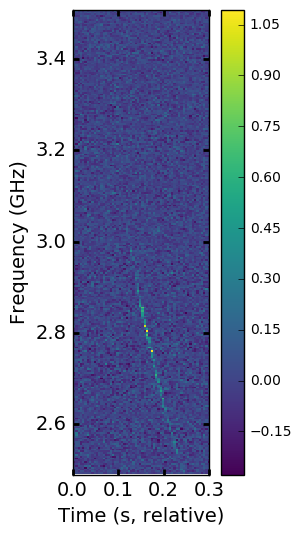
\includegraphics[width=0.25\columnwidth]{sgram_57623.png}
  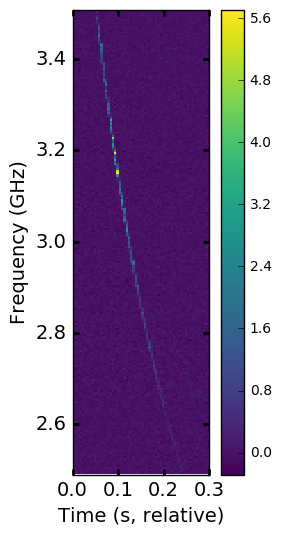
\includegraphics[width=0.25\columnwidth]{sgram_57633_scan7.png}
  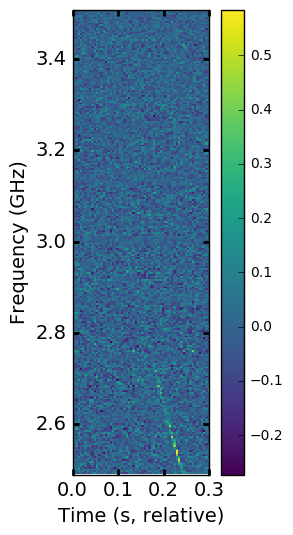
\includegraphics[width=0.25\columnwidth]{sgram_57633_scan13.png}
 \end{minipage}

 \begin{minipage}{2\columnwidth}
  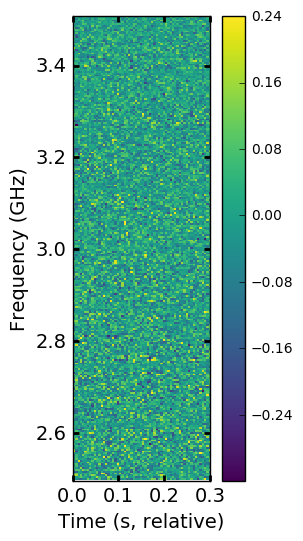
\includegraphics[width=0.25\columnwidth]{sgram_57638.png}
  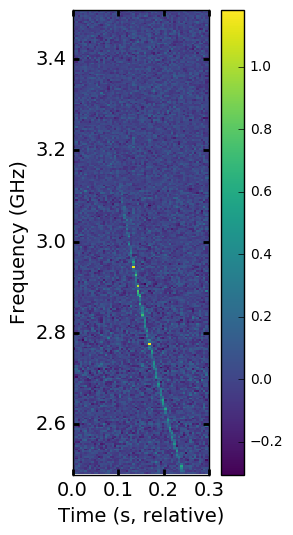
\includegraphics[width=0.25\columnwidth]{sgram_57643.png}
  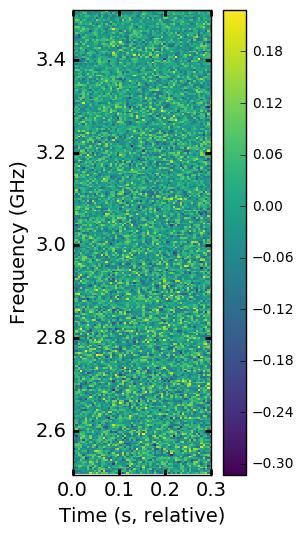
\includegraphics[width=0.25\columnwidth]{sgram_57645.png}
 \end{minipage}

 \begin{minipage}{2\columnwidth}
  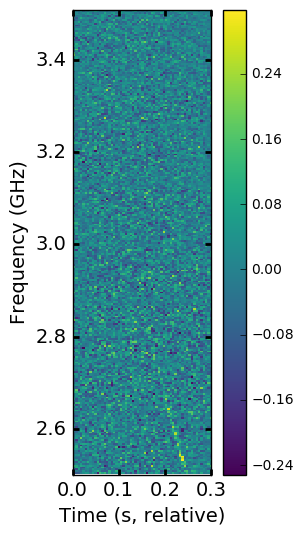
\includegraphics[width=0.25\columnwidth]{sgram_57646.png}
  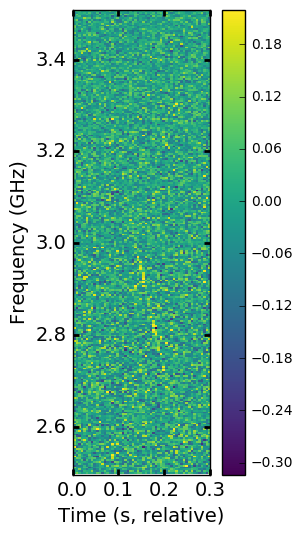
\includegraphics[width=0.25\columnwidth]{sgram_57648.png}
  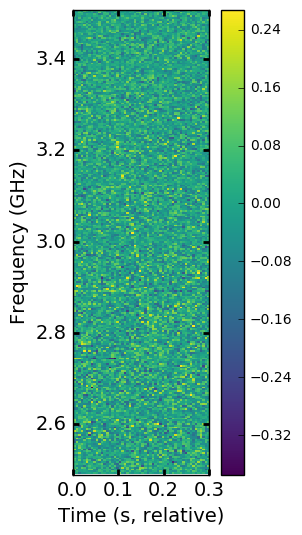
\includegraphics[width=0.25\columnwidth]{sgram_57649.png}
 \end{minipage}
 \caption{Spectrograms (time vs frequency intensity maps) for all nine VLA bursts. Note that bursts are detected in 5~ms images generated from dedispersed visibilities. **NOT SURE WHY ONE FIG LARGER**
 \label{fig:sgram}}
\end{center}
\end{figure*}

\section{Results}

\subsection{Dispersion}

After detection, we refined the analysis of each burst offline. We used a fine dispersion grid to find the best-fit DM for each burst.

Table?
57623 (DM$=561$ pc cm$^{-3}$)
57633, Scan 7 (DM$=554$ pc cm$^{-3}$)
57633, Scan 13 (DM$=559$ pc cm$^{-3}$)
57638 (DM$=554$ pc cm$^{-3}$)
57643 (DM$=559$ pc cm$^{-3}$)
57645 (DM$=572$ pc cm$^{-3}$)
57646 (DM$=573$ pc cm$^{-3}$)
57648 (DM$=559$ pc cm$^{-3}$)
57649 (DM$=552$ pc cm$^{-3}$).

Dispersion measure changes between bursts significant?

\subsection{Spectra}

Burst spectra are shown in Figure \ref{fig:spec}...

\begin{figure*}[h!]
\begin{center}
 \begin{minipage}{2\columnwidth}
  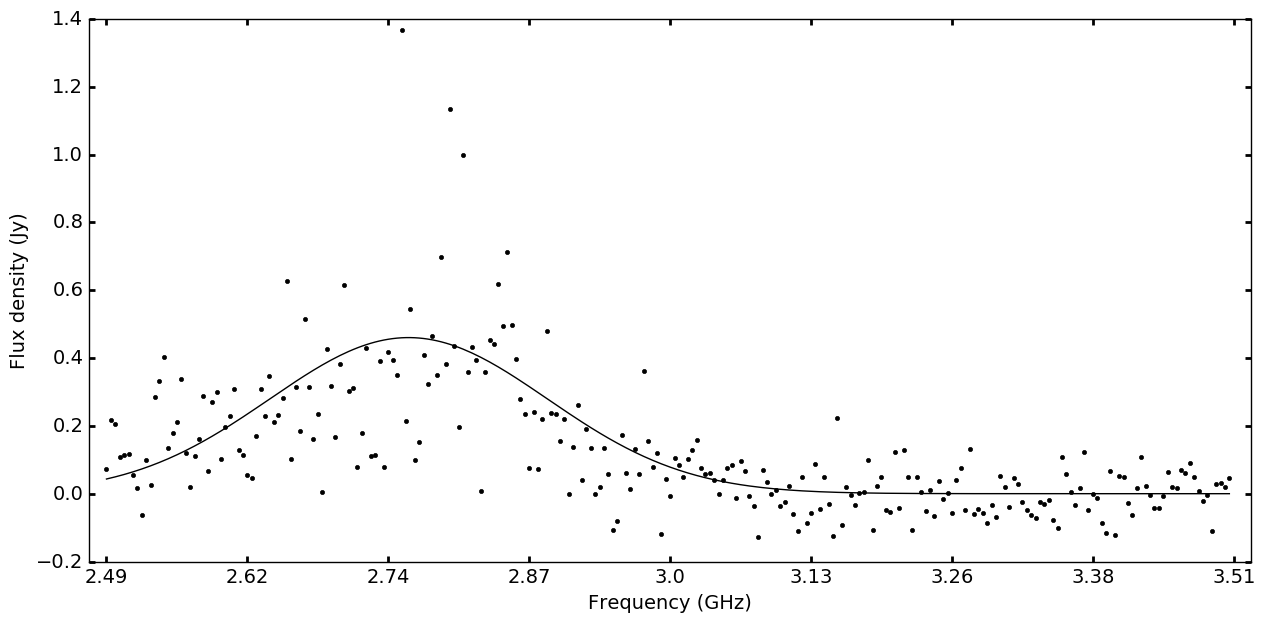
\includegraphics[width=0.3\columnwidth]{spec_57623.png}
  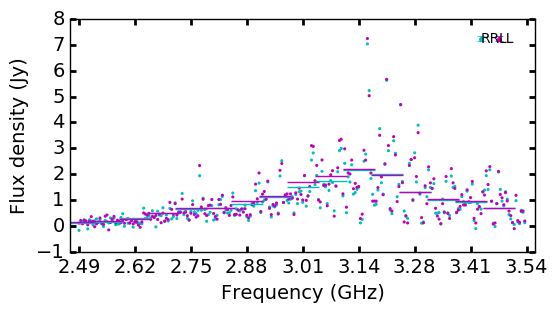
\includegraphics[width=0.3\columnwidth]{spec_57633_scan7.png}
  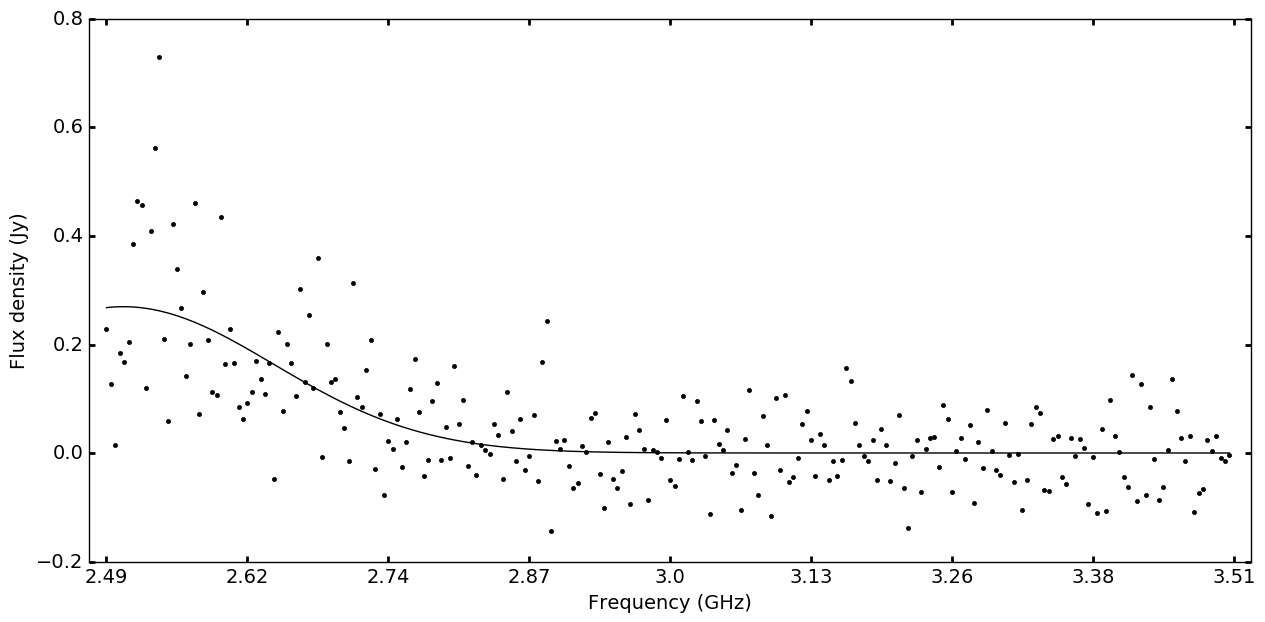
\includegraphics[width=0.3\columnwidth]{spec_57633_scan13.png}
 \end{minipage}

 \begin{minipage}{2\columnwidth}
  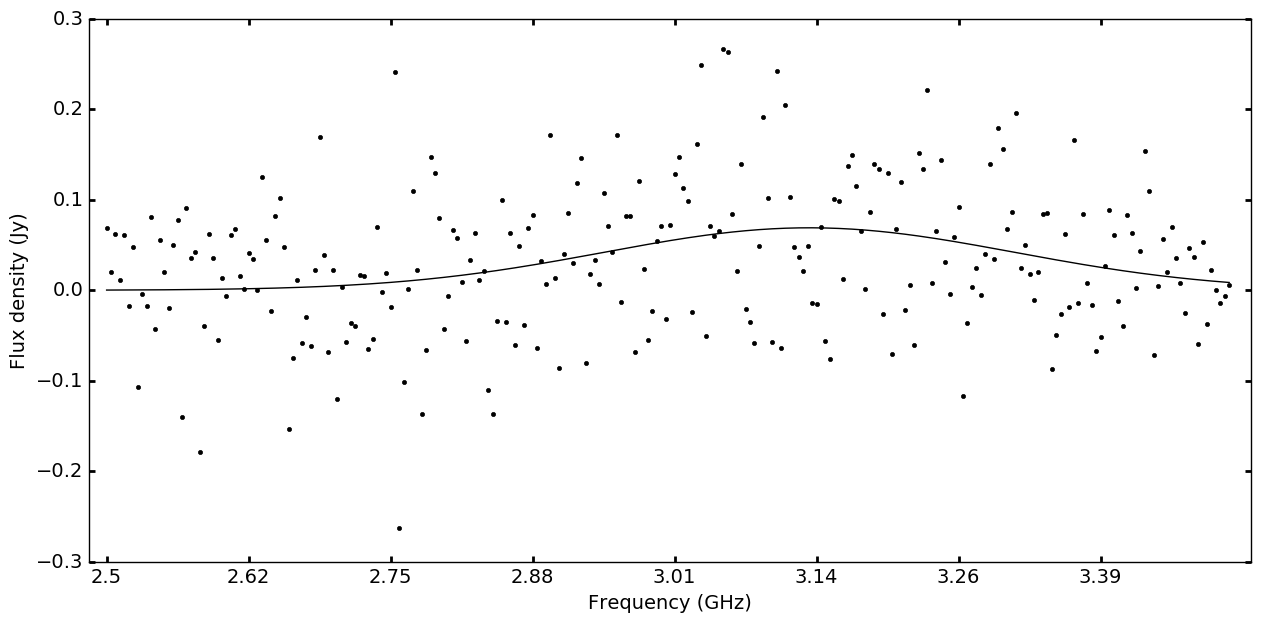
\includegraphics[width=0.3\columnwidth]{spec_57638.png}
  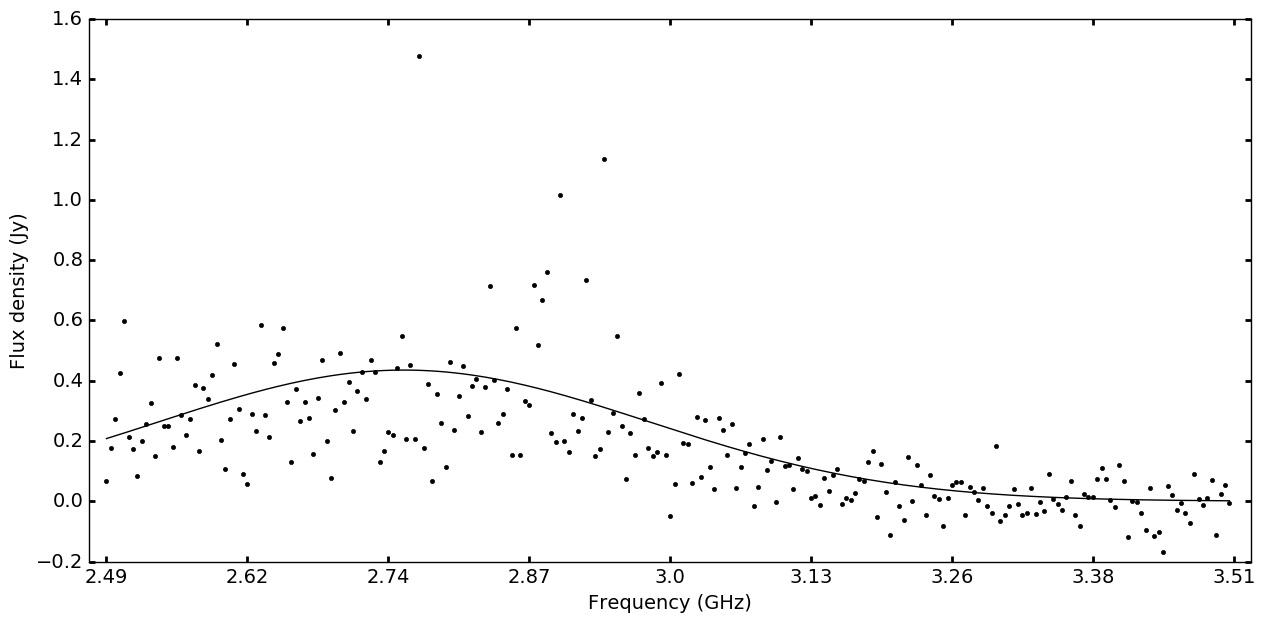
\includegraphics[width=0.3\columnwidth]{spec_57643.png}
  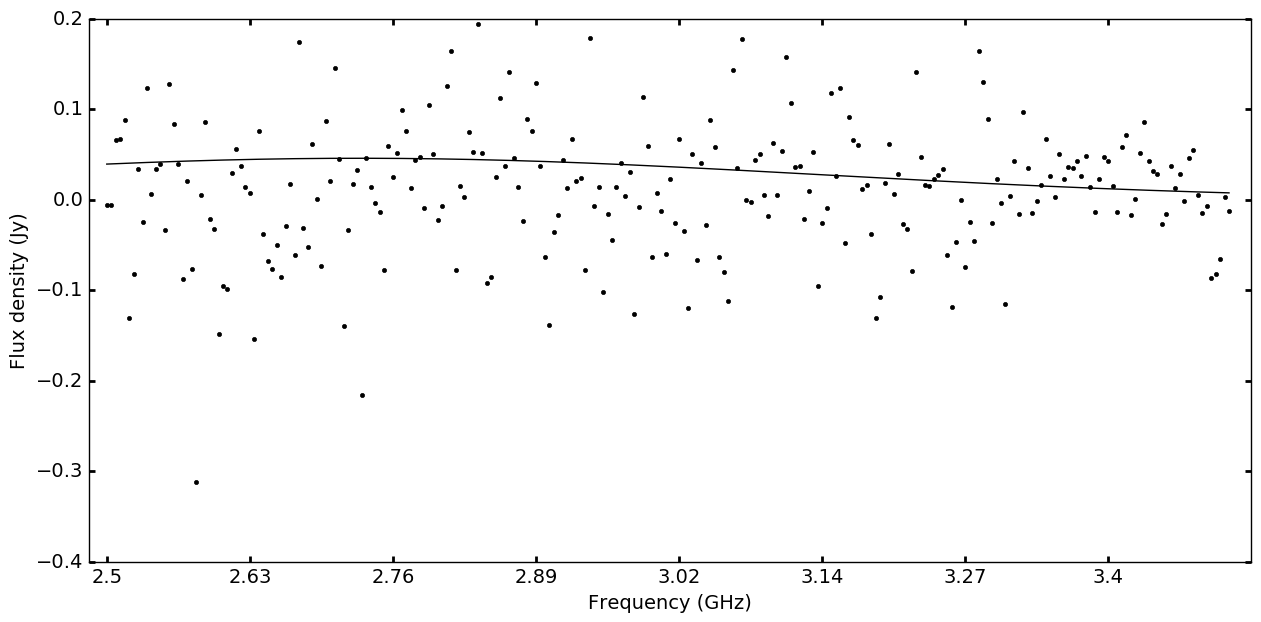
\includegraphics[width=0.3\columnwidth]{spec_57645.png}
 \end{minipage}

 \begin{minipage}{2\columnwidth}
  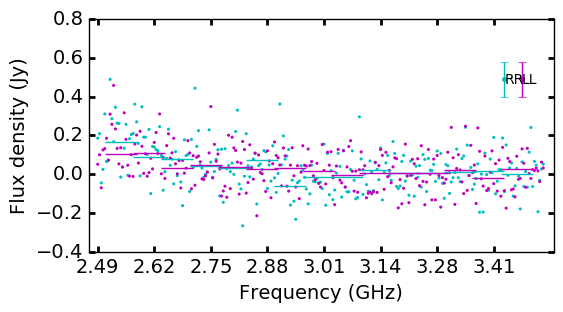
\includegraphics[width=0.3\columnwidth]{spec_57646.png}
  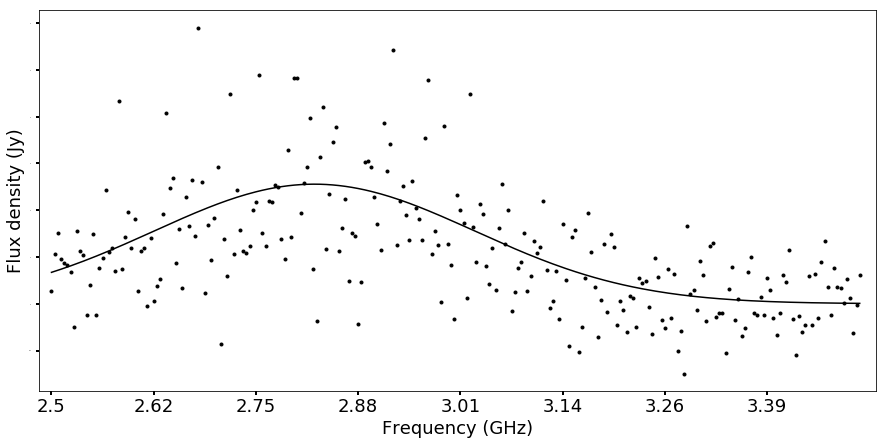
\includegraphics[width=0.3\columnwidth]{spec_57648.png}
  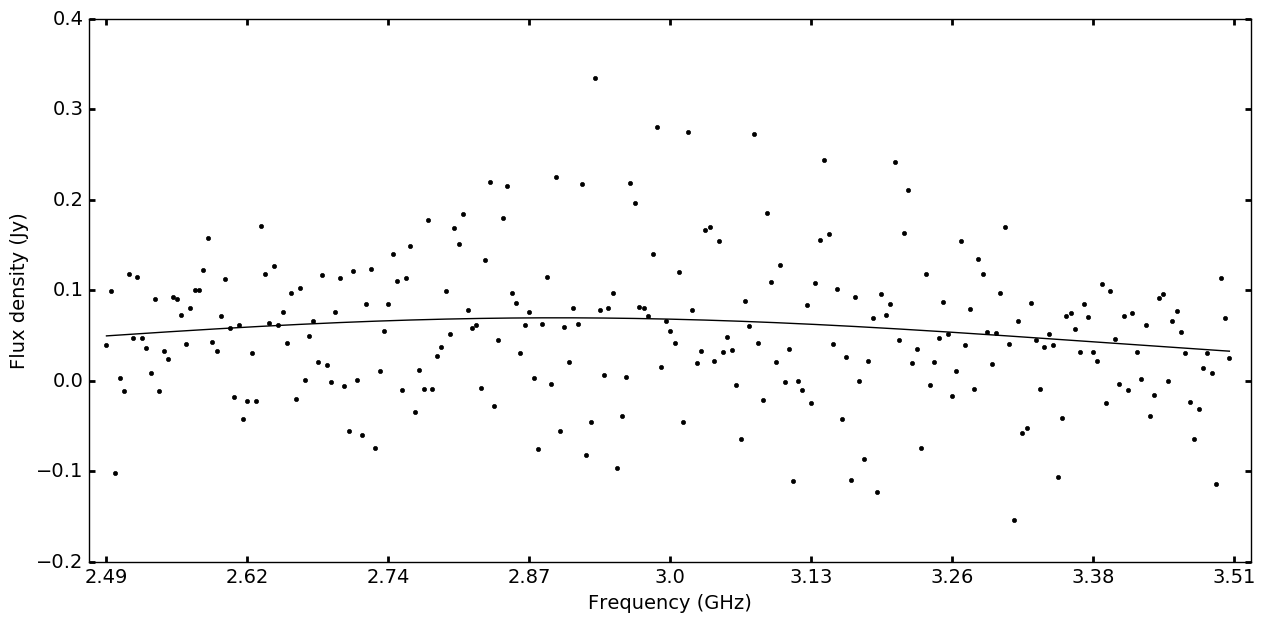
\includegraphics[width=0.3\columnwidth]{spec_57649.png}
 \end{minipage}
\caption{Spectra of nine bursts seen by the VLA from 2.5 to 3.5~GHz.  **LABELS ALL SAME FREQ. SOME SHOULD START HIGHER FOR DROPPED CHANNELS**
 \label{fig:spec}}
\end{center}
\end{figure*}


\subsection{Circular Polarization}

The VLA S-band recievers natively measure circular polarization. The fast VLA interferometric data recorded only dual-circular visibilities and did not perform polarimetric calibration, so only crude polarimetric constraints are possible and only on circular polarization.

Can variation in circular pol between bursts be caused by beam-dependent effects? If not, then we can claim some modest circular pol that varies burst-to-burst.

\subsection{Brightness Distribution}

The bursts seen by the VLA range in significance from 10 to 150$\sigma$. Offline analysis for flux scale...

Figure \ref{fig:logns} shows the flux distribution of the nine VLA bursts. Flatness...

\begin{figure}[htb]
\begin{center}
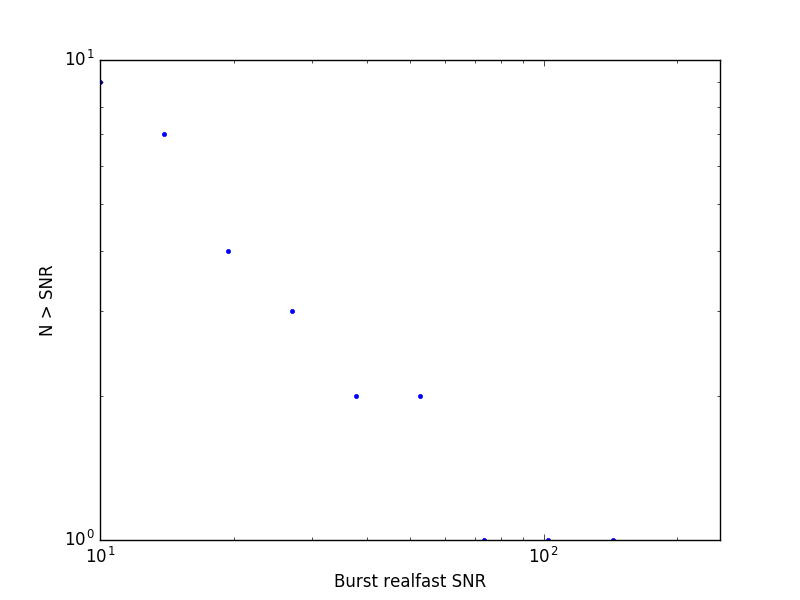
\includegraphics[width=0.9\columnwidth]{logns}
\caption{Log N -- Log SNR distribution of real-time detections of FRB 121102.
\label{fig:logns}}
\end{center}
\end{figure}

Doubts were cast on the first FRB detection (``Lorimer burst'') due to its unusually high brightness. The lack of lower-significance detections suggested that this burst was unlikely to be part of any astrophysical population...

\subsection{Temporal Statistics}

Burst detections were made very inhomogenously though the roughly 60 hours of observing toward FRB 121102. In the first $\sim8$\ hours of observing at L-band and the first $\sim25$\ hours observing at S-band no bursts were detected. Finally, in the last $\sim27$ hours of S-band observing, all nine bursts were detected. Data quality are relatively high and RFI did not significantly impact sensitivity, so the inhomogeneous burst distribution not an observational artifact.

\section{discussion}

\subsection{Connection to Overall FRB Population}

Flat luminosity distribution of FRB121102 and overall population

Does local (100 Mpc) population with flat luminosity distribution reproduce observed properties? Imagine also how log N/log S cut-offs and scattering biases the intrinsic into the observed distribution (Macquart and Johnston)

Discussion of ``red spectrum'' and Connor \& Pen. Bursts predict bursts therefore repetition constraints of other FRBs are likely weaker than claimed...

Intrinsic versus refractive scintillation

Constraints on repetition assuming "red spectrum" for whole population. Simulation using observed burst temporal statistics...


\subsection{Emission Physics and Burst Energetics}



\subsection{Observing Strategies}

Targeting known FRBs is optimal

Wide, low-sensitivity searches are best way to conduct a blind search

\section{Conclusions}



\bibliographystyle{apj}

\section*{Acknowledgements}
We thank ...
This project was supported by the University of California Office of the President under Lab Fees Research Program Award 237863. The National Radio Astronomy Observatory is a facility of the National Science Foundation operated under cooperative agreement by Associated Universities, Inc. 

\bibliography{fasttrants.bib}

%\begin{figure}[htb]
%\begin{center}
%\includegraphics[width=0.9\columnwidth]{}
%\caption{
%\label{fig:name}}
%\end{center}
%\end{figure}

%\begin{table}
%\caption{Caption}
%\footnotesize
%\centering
%\begin{tabular}{l|cc|cc|c}
%\hline
%Field       & RA          & Dec   & Lon. & Lat.     & Time \\
%            & \multicolumn{2}{|c|}{(J2000)}  & \multicolumn{2}{|c|}{(Galactic; deg)} & (hrs) \\ \hline
%RA02        & 2:27:53  &  +9:13:24 & 159.0 & --46.8    & 26.25 \\
%PSR J2248-0101 & 22:48:27 & --1:1:48 & 69.3 & --50.6 & 6.5 \\ \hline
%\end{tabular}
%\label{fields}
%\end{table} 

\end{document}

